\documentclass{beamer}
\usepackage[english]{babel}
\usepackage{calc}
\usepackage[absolute,overlay]{textpos}
\mode<presentation>{\usetheme{tud}}



\usepackage{tikz}
\usetikzlibrary{positioning,arrows}

\tikzset{
  block/.style={
    draw,
    rectangle,
    minimum height=1cm,
    minimum width=1cm,
    align=center
  },
  subblock/.style={
    draw,
    rectangle,
    minimum height=.75cm,
    minimum width=1.5cm,
    align=center
  },
  line/.style={->,>=latex},
  LED/.style={draw,circle,append after command={
        [shorten >=\pgflinewidth, shorten <=\pgflinewidth,]
        %(\tikzlastnode.north) edge (\tikzlastnode.south)
        %(\tikzlastnode.east) edge (\tikzlastnode.west)
        }
    },
  dot/.style={draw,circle,minimum size=2mm,inner sep=0pt,outer sep=0pt,fill=black}
}

\usepackage{pifont}% http://ctan.org/pkg/pifont
\newcommand{\cmark}{\ding{51}}%
\newcommand{\xmark}{\ding{55}}%



\usepackage{epstopdf}




\title[Mid-term Presentation]{Leveraging VLC for energy }
\subtitle{disaggregation in Smart Buildings}
\institute[TU Delft]{Delft University of Technology}
\author{Johnny Verhoeff}
\date{\today}

% Insert frame before each subsection (requires 2 latex runs)
\AtBeginSubsection[] {
	\begin{frame}<beamer>\frametitle{\titleSubsec}
		\tableofcontents[currentsection,currentsubsection]  % Generation of the Table of Contents
	\end{frame}
}
% Define the title of each inserted pre-subsection frame
\newcommand*\titleSubsec{Next Subsection}
% Define the title of the "Table of Contents" frame
\newcommand*\titleTOC{Outline}

% define a symbol which can be removed if you don't need it
\newcommand{\field}[1]{\mathbb{#1}}
\newcommand{\Zset}{\field{Z}}

\begin{document} {
	% remove the next line if you don't want a background image
	\usebackgroundtemplate{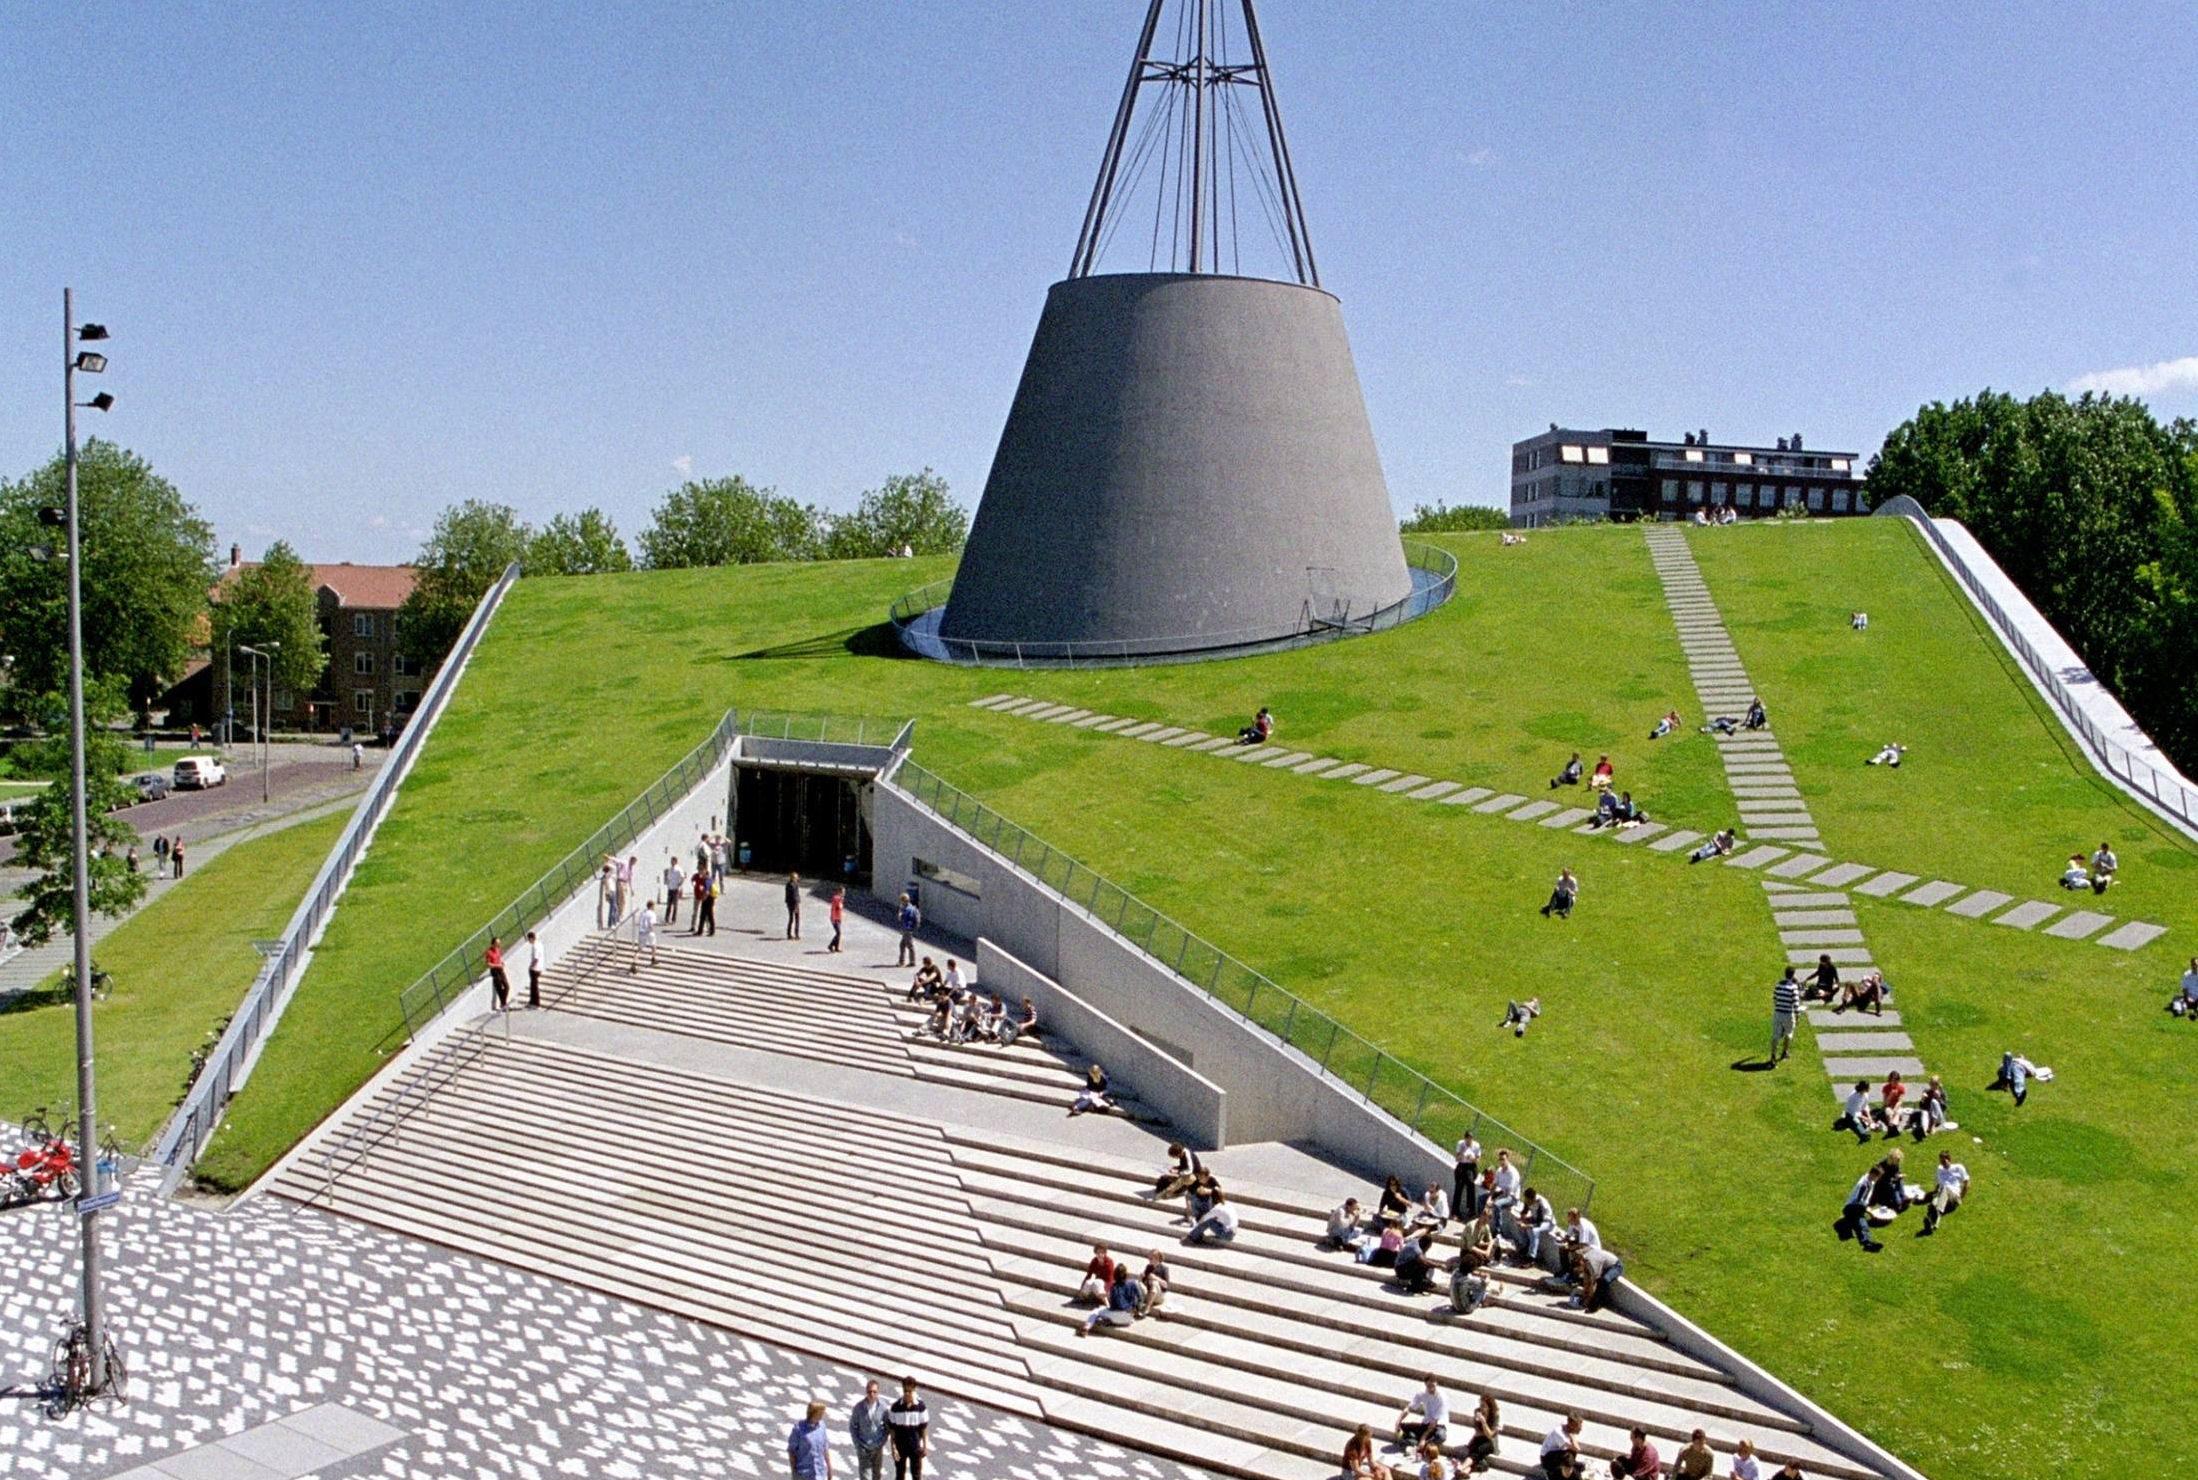
\includegraphics[width=\paperwidth,height=\paperheight]{images/background-titlepage.jpg}}%
	\setbeamertemplate{footline}{\usebeamertemplate*{minimal footline}}
	\frame{\titlepage}
}

\beamertemplatenavigationsymbolsempty
%\setbeamertemplate{navigation symbols}{}

\setbeamertemplate{caption}{\raggedright\insertcaption\par}

%{\setbeamertemplate{footline}{\usebeamertemplate*{minimal footline}}
%\begin{frame}\frametitle{\titleTOC}
%	\tableofcontents
%\end{frame}
%}

%\section{First Section}
%\subsection{Section 1 - Subsection 1}


	%intro
	\begin{frame}\frametitle{Energy Disaggregation}

		Energy consumption is a most pressing issue.

		\begin{itemize}

			\item To reduce it, understanding the usage of that energy is needed.

			\item Smart-meter can disaggregate the energy usage in a household.

			\item This is done by recognizing the unique signatures of appliances.

		\end{itemize}

		\begin{figure}[t]
			\centering
			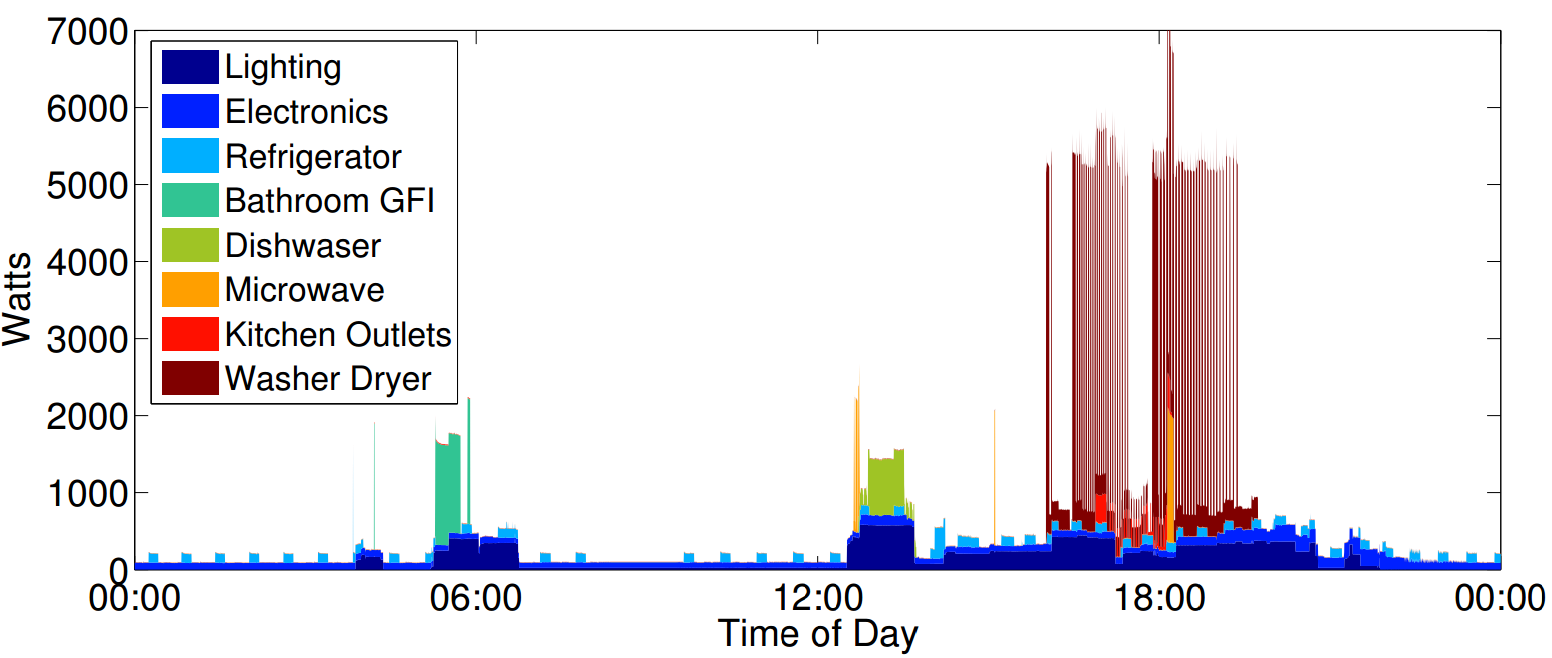
\includegraphics[width=0.7\textwidth]{../chapters/introduction-chapters/energy-consumption-house.png}
		\end{figure}

		% For example here we can see the aggregated energy from a household during a day.
		% With the different colors it is indicated what appliance is being used at what time.
		% In the blue we can see 'lighting' as a constant consumer but it can not disaggregate which individual lights are on.

	\end{frame}






	\begin{frame}\frametitle{Lighting Energy}

		Individual lights cannot be disaggregated (yet).

		\begin{itemize}

			\item The reason: Lighting does not have a unique signature. %Which HVAC for example does have.

			\item Instead there are many lights with the same signature.

			\item Still important to be able to disaggregate individual lights. % Because it is the third largest power consumer in an average household.

		\end{itemize}


	\end{frame}





	\begin{frame}\frametitle{VLC}

		VLC is a communication method which uses visible light to transmit data.

		\begin{itemize}

			\item This data will also propagate through the current draw.

			\item By choosing the data carefully, each light can be identified by its unique current draw.

		\end{itemize}

	\end{frame}






	\begin{frame}\frametitle{Encoding}
		%Easiest way to use VLC is with OOK

		Most common way to use VLC with LEDs, is with On-off keying (OOK).

		\begin{itemize}

			\item LEDs will be turning on and off according to the data.

			\item Binary data is 0 and 1 valued.

			\item Correspondence: 0 $\xrightarrow{}$ LED off, 1 $\xrightarrow{}$ LED on.

		\end{itemize}
	\end{frame}


	\begin{frame}\frametitle{Overview}

		%Smart-meter will measure aggregated current draw of all LEDs.

		\begin{figure}
			\centering
			\resizebox {0.8\textwidth} {!} {
				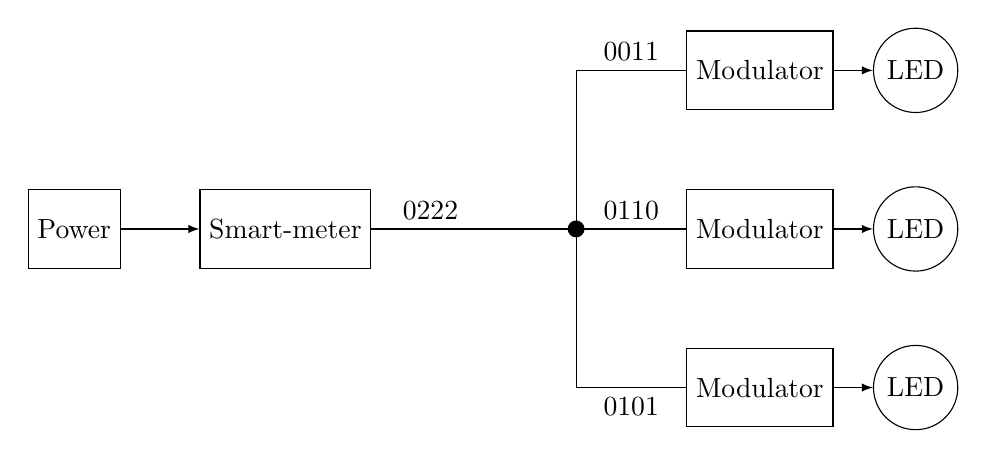
\begin{tikzpicture}

					\node[block] (smart_meter) {Smart-meter};	

					\node[block, left = 1cm of smart_meter] (power) {Power};	
					\draw[line] (power.east) -- (smart_meter.west) node [midway, right] {};		

					% second mod.
					\node[block, right = 4cm of smart_meter] (second_modulator) {Modulator};
					\node[LED, right = 0.5cm of second_modulator] (second_led) {LED};
					\draw[line] (second_modulator.east) -- (second_led.west) node [midway, right] {};

					% first mod.
					\node[block, above = 1cm of second_modulator] (first_modulator) {Modulator};
					\node[LED, right = 0.5cm of first_modulator] (first_led) {LED};
					\draw[line] (first_modulator.east) -- (first_led.west) node [midway, right] {};

					% third mod.
					\node[block, below = 1cm of second_modulator] (third_modulator) {Modulator};
					\node[LED, right = 0.5cm of third_modulator] (third_led) {LED};
					\draw[line] (third_modulator.east) -- (third_led.west) node [midway, right] {};

					\node[dot, right = 2.5cm of smart_meter] (CP) {};

					\draw (smart_meter.east) -- (CP) node [pos=0.3, above] {0222};

					\draw (CP) |- (first_modulator.west) node  [pos=0.75, above] {0011};
					\draw (CP) |- (second_modulator.west) node [pos=0.75, above] {0110};
					\draw (CP) |- (third_modulator.west) node  [pos=0.75, below] {0101};

				\end{tikzpicture}
			}
		\end{figure}

		\begin{itemize}

			\item What data to use to modulate the LEDs ?

			\item Which hardware to use for the modulator and smart-meter ?

			\item Evaluate the solutions.

		\end{itemize}

	\end{frame}




	\begin{frame}\frametitle{CDMA}
		Metrics to consider of a CDMA sequence:

		\begin{itemize}

			\item Length of the sequence. % each chip of the code has to be transmitted and therefor takes time.

			\item Number of sequences with the same length. % determines scalability of the system.


			\item Correlation: A measure for determining how much a sequence is similar to another sequence.
			\begin{itemize}

				\item Auto-correlation: Should have one peak, to identify a particular sequence. % To determine if a particular LED's signature is in the received signal.

				\item Cross-correlation: Should be as small as possible, to limit the amount of interference. % Determines the interference that the LEDs have on each other. 
				%Too much interference and information gets lost.
			\end{itemize}

		\end{itemize}
	\end{frame}


	\begin{frame}\frametitle{Comparison CDMA Sequences}
		

		% these are the sequences which I have investigated 
		% The orthogonal sequences work really well when the transmitters can be synchronized.
		% But due to the nature of lights, they will transmit a-synchronous.
		% The other sequences work in a-synch circumstances.
		% Where the Gold seq. work slight better and have better scalability.


		\begin{table}
			\centering
			\resizebox {\textwidth} {!} {
				\begin{tabular}{ | l | l | l | l | }

					\hline
															& Orthogonal Seq. 			& PN Seq.						& Gold Seq.				\\ \hline
			Synchronous	Transmission						& \cmark					& \cmark						& \cmark				\\ \hline
			A-synchronous Transmission						& \xmark					& \cmark						& \cmark				\\ \hline
			Peaks auto-correlation (synchronous)			& 1							& 1								& 1						\\ \hline
			Peaks auto-correlation (a-synchronous)			& $> 1$						& 1								& 1						\\ \hline
			Low cross-correlation (synchronous)				& \cmark					& \cmark						& \cmark				\\ \hline
			Low cross-correlation (a-synchronous)			& \xmark					& \cmark						& \cmark				\\ \hline
			Math. bounded cross-correlation (synchronous)	& \cmark					& \xmark						& \cmark				\\ \hline
			Math. bounded cross-correlation (a-synchronous)	& \xmark					& \xmark						& \cmark				\\ \hline
			Scalability ($C \propto L$)						& \cmark					& \xmark						& \cmark				\\ \hline		


				\end{tabular}
			}

		\end{table}
	\end{frame}



	\begin{frame}\frametitle{Mapping Problem}
		CDMA sequences are designed for and used in (wireless) telecommunications.

		\begin{itemize}

			\item Due to the use of analog radio signal the symbols are +1 and -1.

			\item LEDs can have the two state: Off (0) and On (1).

			\item Mapping between these two sets of symbols must take place.

			\item This mapping alters the way the correlation is calculated.

		\end{itemize}
		
	\end{frame}


	\begin{frame}\frametitle{Probabilistic Scheme}
		Cross-correlation is not negligible.

		\begin{itemize}

			\item Cross-correlation is a function of the length of the sequence.

			\item The maximum number of concurrent transmitters $m$ can be calculated, such that no interference will take place. % which will be a function of the length of the sequence.

			\item A probability $p$ is assigned to each transmitter based on the sequence and the time frame and completeness that the user requires.

		\end{itemize}
	\end{frame}





	\begin{frame}\frametitle{Theory To Practice}

		Components for both DC and AC will be investigated: 

		\begin{itemize}

			\item LED modulator

			\item Current sampler (smart-meter)

		\end{itemize}
		
	\end{frame}


	\begin{frame}\frametitle{DC Hardware}

		Modulator: 

		\begin{itemize}

			\item Constant current source

		\end{itemize}

		Current sampler: 

		\begin{itemize}

			\item Burden resistor with an ADC

		\end{itemize}
		
	\end{frame}




	\begin{frame}\frametitle{AC Hardware}

		\begin{figure}
			\centering
			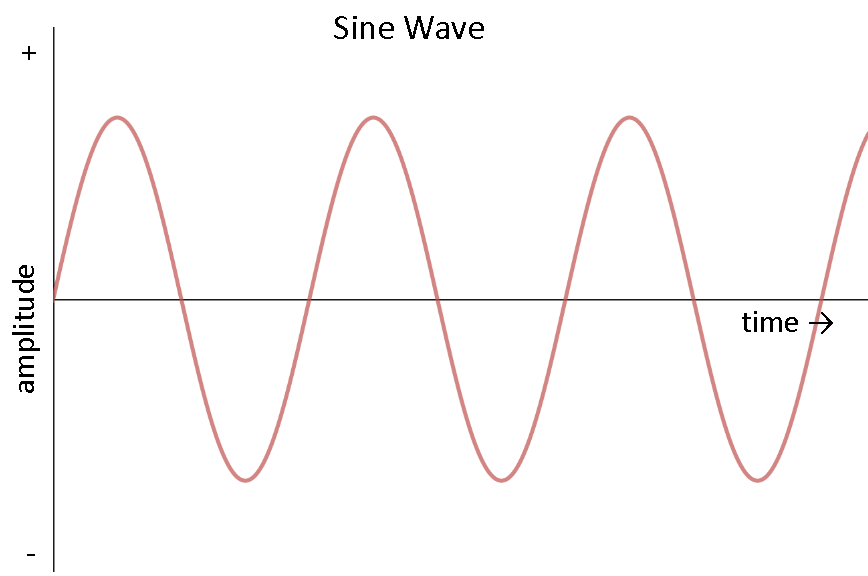
\includegraphics[width=0.6\textwidth]{ac-sine-wave.png}
		\end{figure}

		AC is not like DC: 

		\begin{itemize}

			\item Supplied voltage is not constant.

			\item Supplied voltage will be both positive and negative.

		\end{itemize}

		%Since this is not so easy to deal with as with DC, first other hw was investigated 
		
	\end{frame}

	\begin{frame}\frametitle{AC Hardware}

		\begin{figure}
			\resizebox {0.8\textwidth} {!} {
			  \centering
			  \begin{minipage}[b]{0.48\textwidth}
			    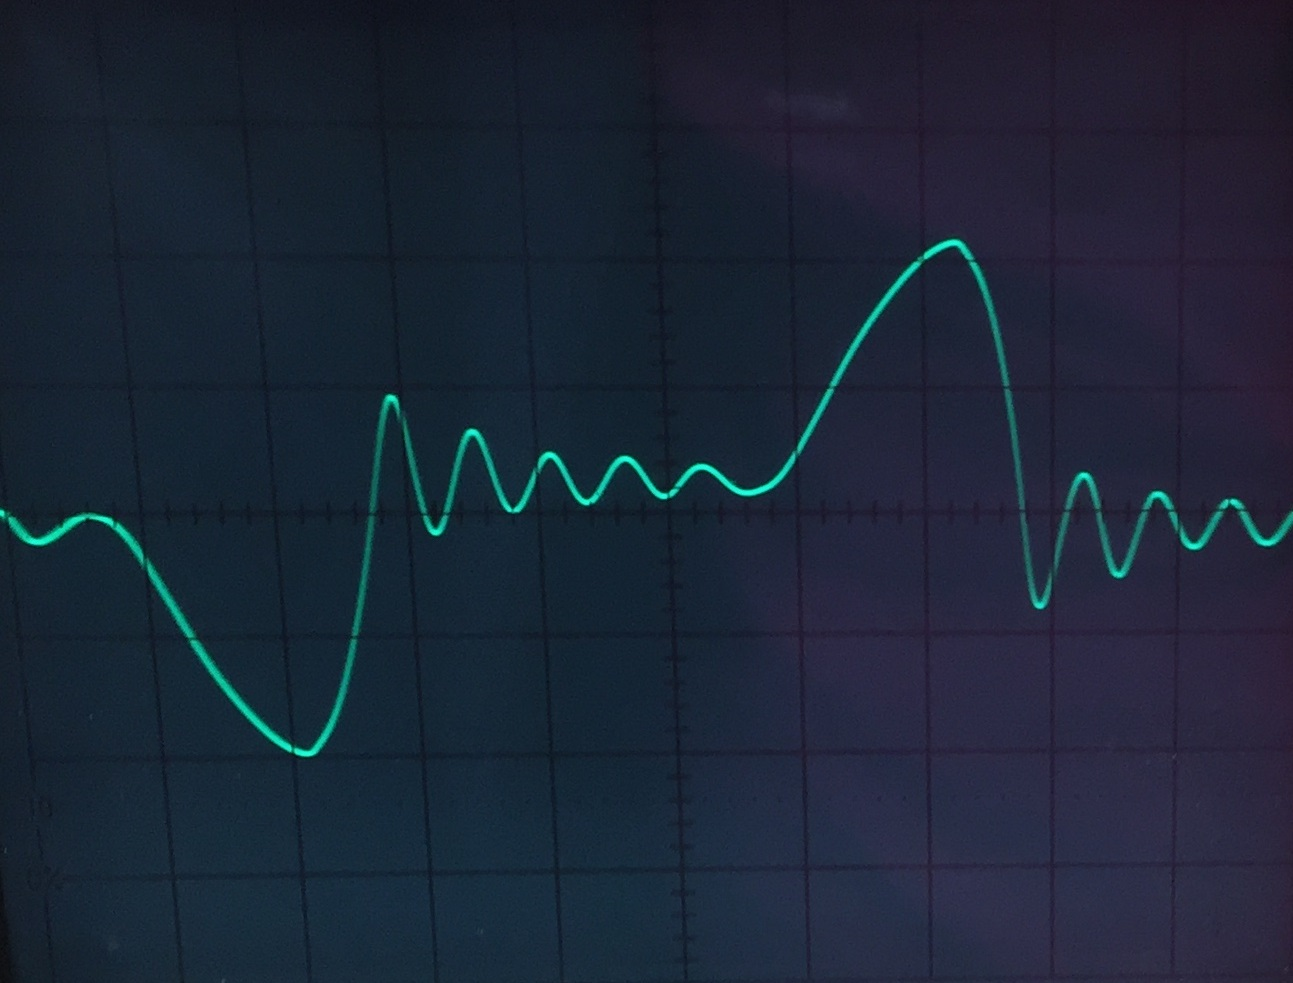
\includegraphics[width=\textwidth]{../chapters/hardware-chapters/smps-current-primary-with-load-cropped.jpg}
			    \caption{SMPS}
			  \end{minipage}
			  \hfill
			  \begin{minipage}[b]{0.4\textwidth}
			    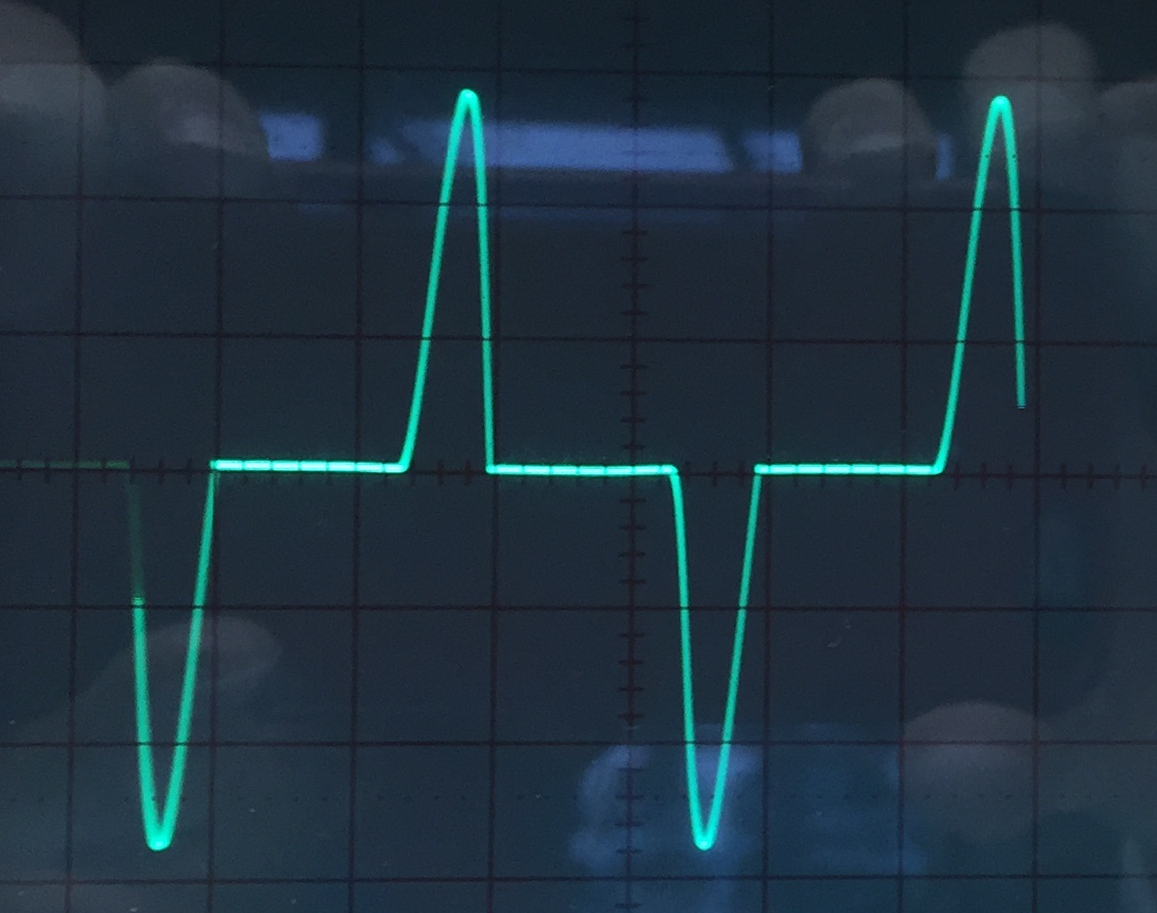
\includegraphics[width=\textwidth]{../chapters/hardware-chapters/commercial-230v-ac-led-on-cropped.png}
			    \caption{Commercial AC LED}
			  \end{minipage}
		  }
		\end{figure}

		These solutions will not yield nice aggregated signals.
		
	\end{frame}

	\begin{frame}\frametitle{AC Hardware}

		Design of the AC LED modulator: 

		\begin{itemize}

			\item AC Voltage is zero crossing:
			\begin{itemize}
				\item Triggering needed to decide when to modulate. %because LEDs need certain amount of voltage before the current starts flowing
			\end{itemize}

			\item AC Voltage is not constant:
			\begin{itemize}
				\item Constant current source for LED. %because varying supplied voltage, but still want flat current curve.
			\end{itemize}


		\end{itemize}

		\begin{figure}
			\resizebox {0.8\textwidth} {!} {
			  \centering
			  \begin{minipage}[b]{0.4\textwidth}
			    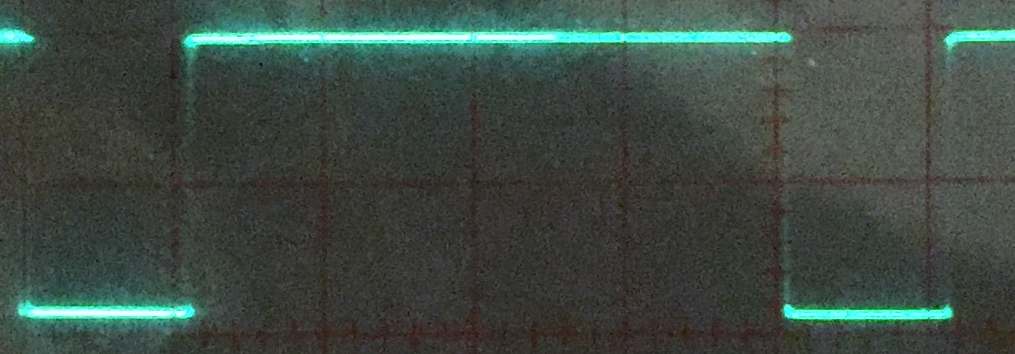
\includegraphics[width=\textwidth]{../chapters/hardware-chapters/triggering-circuit-output-cropped.png}
			    \caption{Triggering output}
			  \end{minipage}
			  \hfill
			  \begin{minipage}[b]{0.4\textwidth}
			    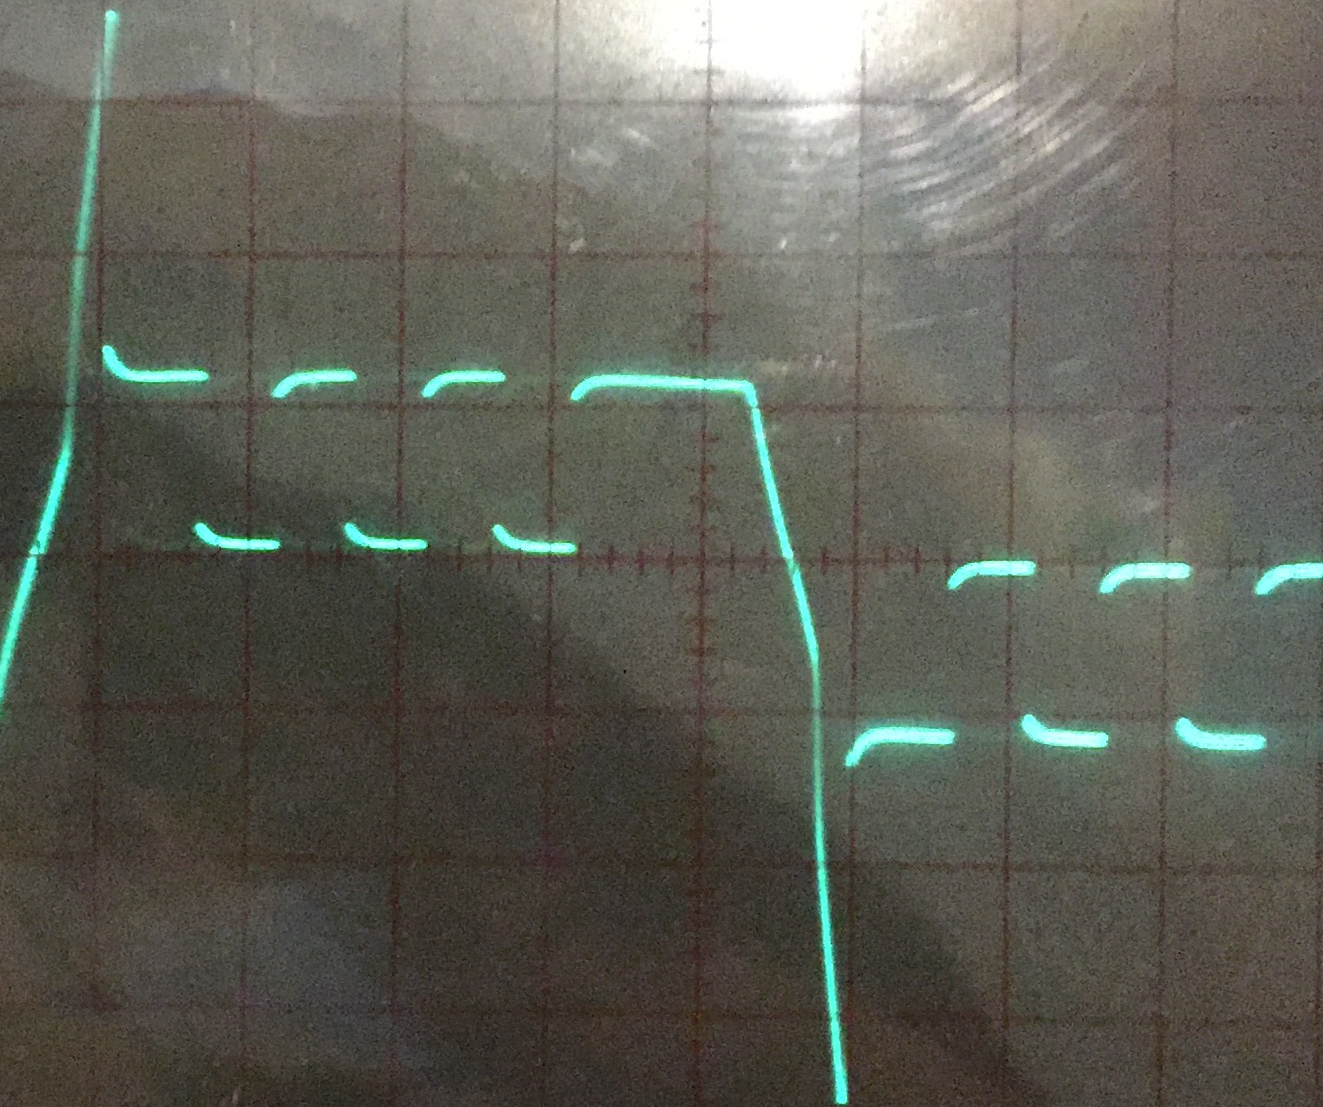
\includegraphics[width=\textwidth]{../chapters/hardware-chapters/current-source-measurement-cropped.png}
			    \caption{Constant current source}
			  \end{minipage}
		  }
		\end{figure}
		
		
	\end{frame}



	\begin{frame}\frametitle{AC Hardware}

		AC Current sampler options:

		\begin{columns}
			\begin{column}{0.48\textwidth}

				\begin{itemize}
					\item Hall effect sensor:

					\begin{itemize}
						\item Sensitivity: 185 mV / A
						\item Noise: 21 mV
						\item Output: 15 W LED yields 12 mV 
					\end{itemize}

					\item Burden resistor:

					\begin{itemize}
						\item Sensitivity: 2800 mV / A
						\item No noise 
						\item Output: 15 W LED yields 183 mV 
						\item Positive and negative voltage output %because of AC, so add a constant voltage to it and feed to an ADC
					\end{itemize}


				\end{itemize}
			\end{column}
			\begin{column}{0.48\textwidth}

				\begin{figure}
					\centering
					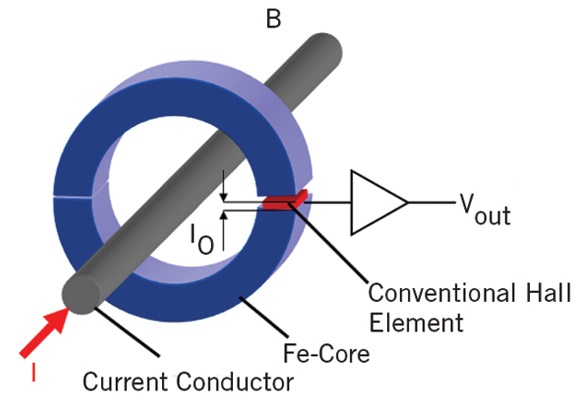
\includegraphics[width=0.8\textwidth]{hall-effect-sensing}
				\end{figure}

			\end{column}
		\end{columns}


		

		
		
	\end{frame}




	\begin{frame}\frametitle{Testbeds}
		

		\begin{itemize}

			\item DC testbed has 6 individual controllable LEDs + current sampler. [Pic]

			\item AC testbed has 3 individual controllable LEDs + current sampler. [Pic]

		\end{itemize}
	\end{frame}



	\begin{frame}\frametitle{Evaluation DC Testbed}

		\begin{figure}[!tbp]
		  \centering
		  \begin{minipage}[b]{0.49\textwidth}
		    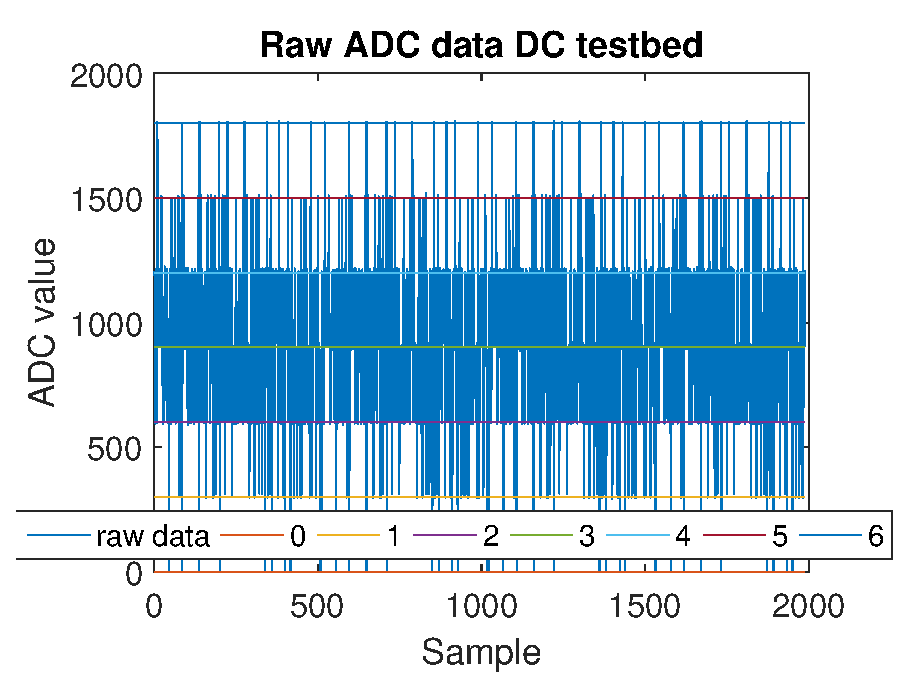
\includegraphics[width=\textwidth]{../chapters/evaluation-chapters/hardware/dc/raw-dc-testbed-adc-data-n=9.eps}
		  \end{minipage}
		  \hfill
		  \begin{minipage}[b]{0.49\textwidth}
		    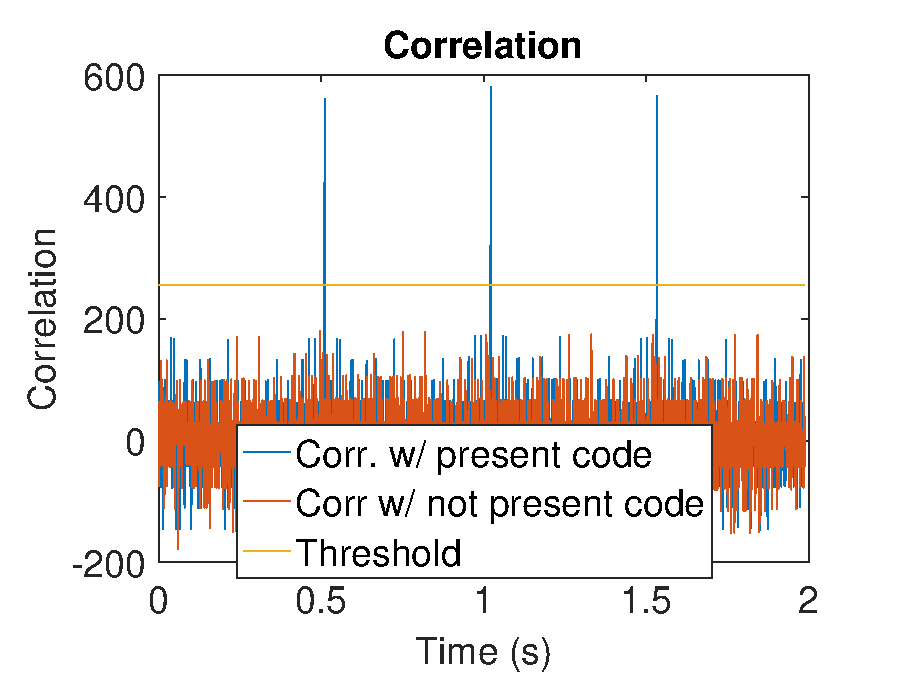
\includegraphics[width=\textwidth]{../chapters/evaluation-chapters/hardware/dc/correlation-dc-testbed-n=9.eps}
		  \end{minipage}
		\end{figure}

		% On the left hand side the raw data captured by the ADC can be seen.
		% The 6 LEDs are all modulating according to the code sequences that they were given.

		% On the right hand side the correlation results can be seen with two code sequences
		% One sequence which is also used for one of the LEDs and one which is not being used
		% We can only see peaks for the correct code.

	\end{frame}



	\begin{frame}\frametitle{Evaluation AC Testbed}

		\begin{figure}[!tbp]
		  \centering
		  \begin{minipage}[b]{0.4\textwidth}
		    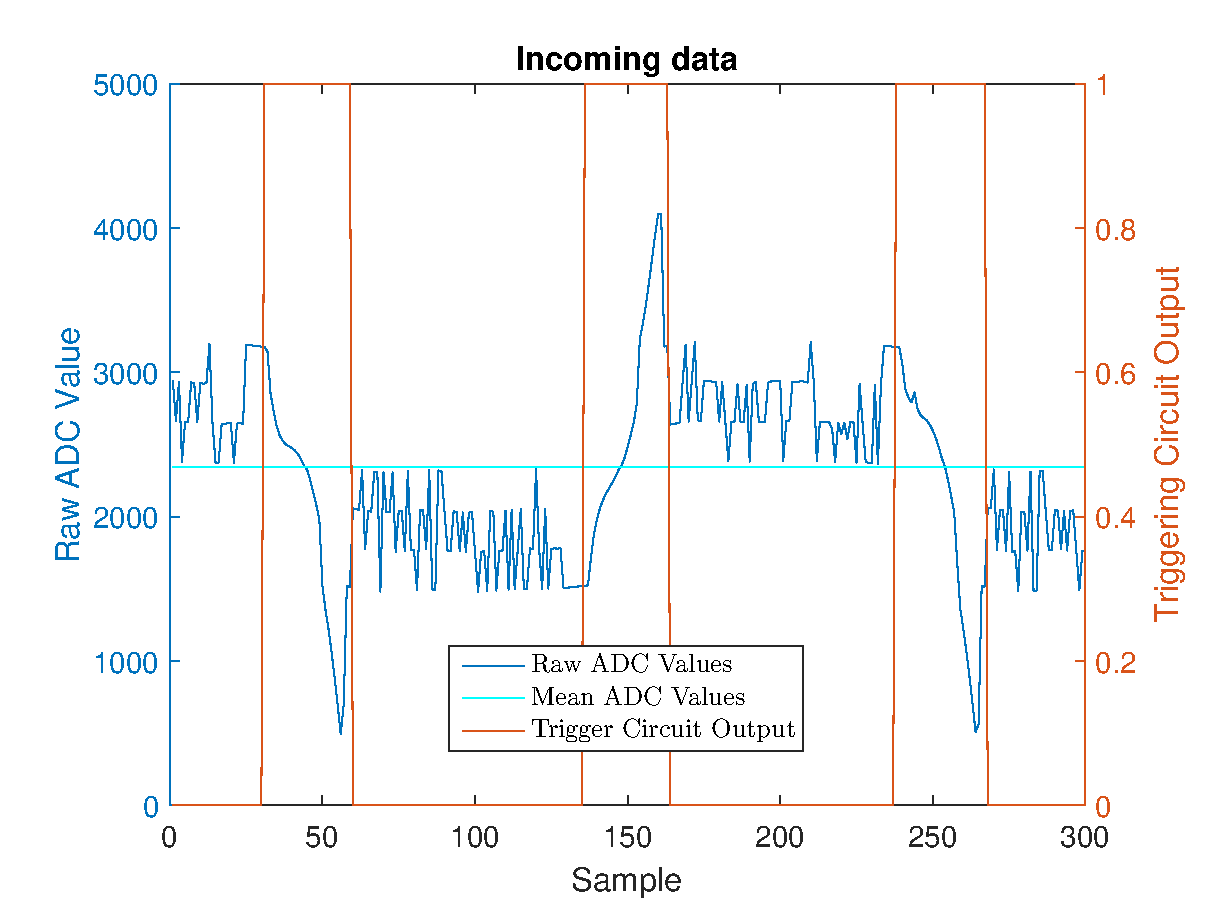
\includegraphics[width=\textwidth]{../chapters/evaluation-chapters/hardware/ac/raw-ac-testbed-adc-data.eps}
		  \end{minipage}
		  \hfill
		  \begin{minipage}[b]{0.4\textwidth}
		    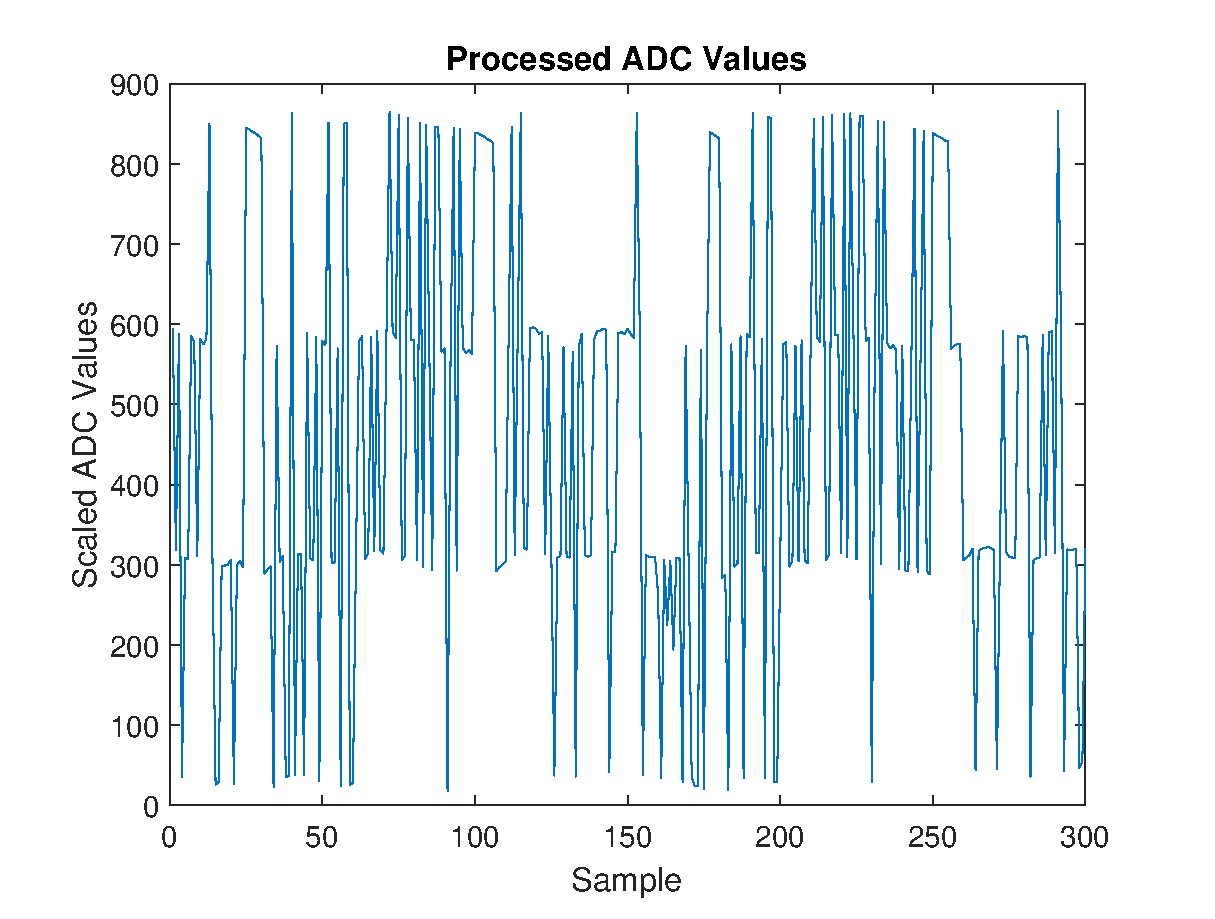
\includegraphics[width=\textwidth]{../chapters/evaluation-chapters/hardware/ac/processed-ac-testbed-adc-data.eps}
		  \end{minipage}
		  \hfill
		  \begin{minipage}[b]{0.4\textwidth}
		    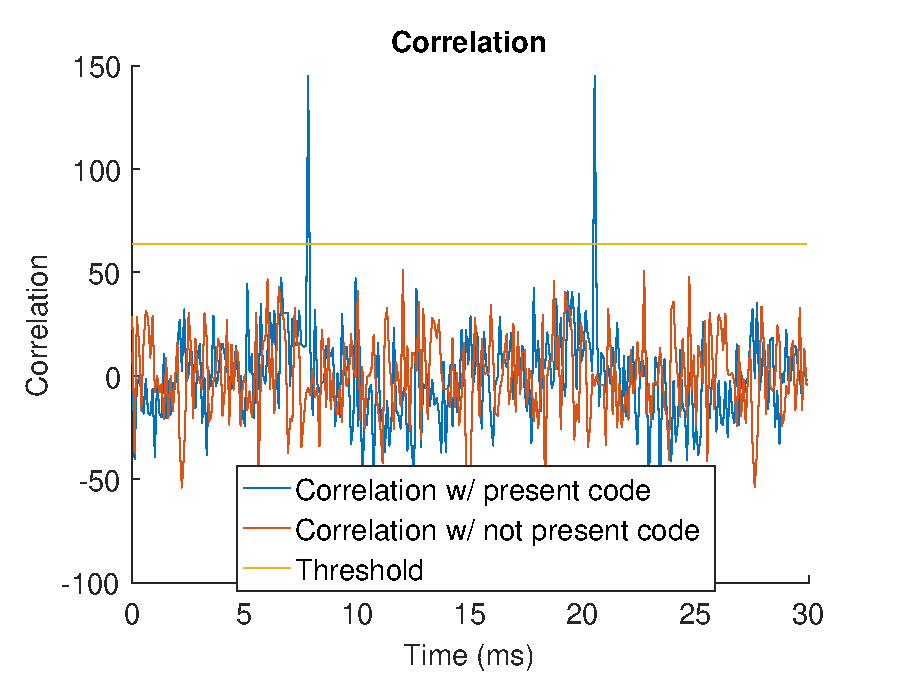
\includegraphics[width=\textwidth]{../chapters/evaluation-chapters/hardware/ac/correlation-ac-testbed.eps}
		  \end{minipage}
		\end{figure}


		% The first figure shows the raw ADC data with the triggering output.
		% This signal is processed to be able to correlate the signal just like with the DC testbed
		% The last figure shows the correlation with a sequence that is present and a sequence that is not present, very similar to the dc testbed.

	\end{frame}







	\begin{frame}\frametitle{Simulation}
		
		To be able to test larger systems, simulations are used.

		Assuming 129 individual LEDs which follow the probabilistic scheme.

	\end{frame}



	\begin{frame}\frametitle{Simulation}
		
		\begin{figure}[t]
			\centering
			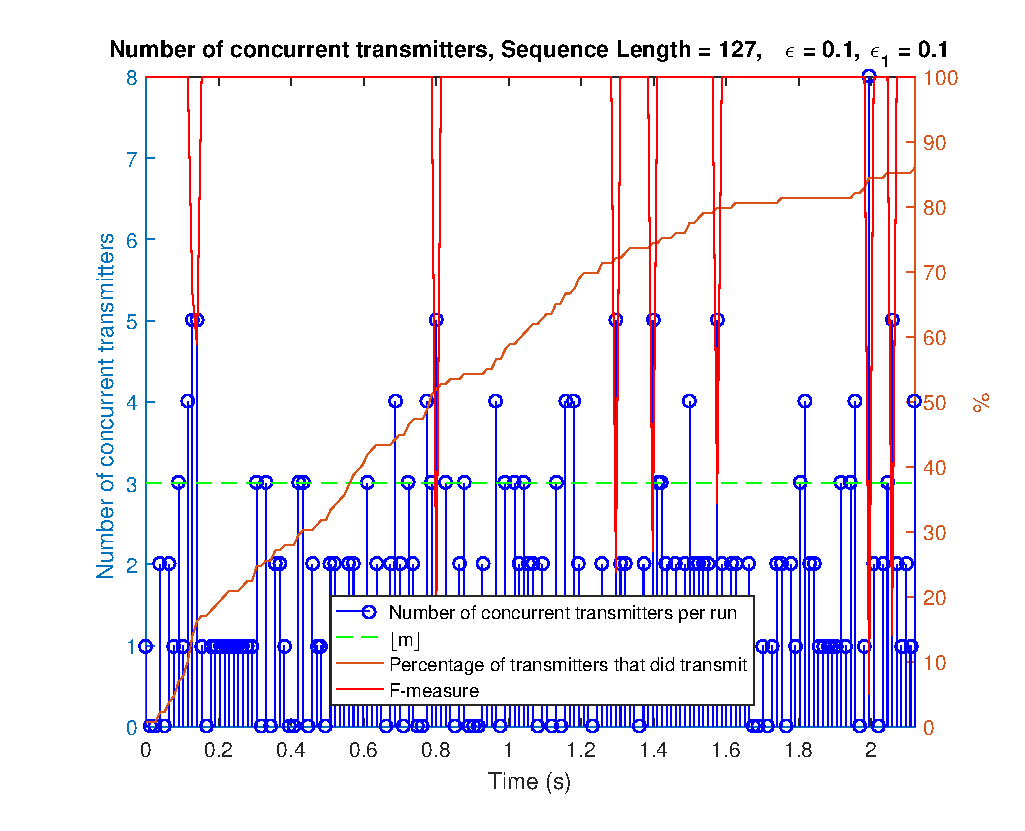
\includegraphics[width=0.8\textwidth]{simulation-1.eps}
		\end{figure}

		% With this probabilistic scheme, the settings are a bit high, which will result in fast times but low completeness and decoding errors.
		% Every time the number of concurrent transmitters goes above the m line, interference MAY happen, below the line everything will be fine, this is proven.
		% WHen the interference happens fp and fn may occur and we see the f-measure drop.
		% for 129 transmitters it takes 2.1 seconds to let 85 % of the transmitters transmit.

	\end{frame}

	\begin{frame}\frametitle{Simulation (2)}
		
		\begin{figure}[t]
			\centering
			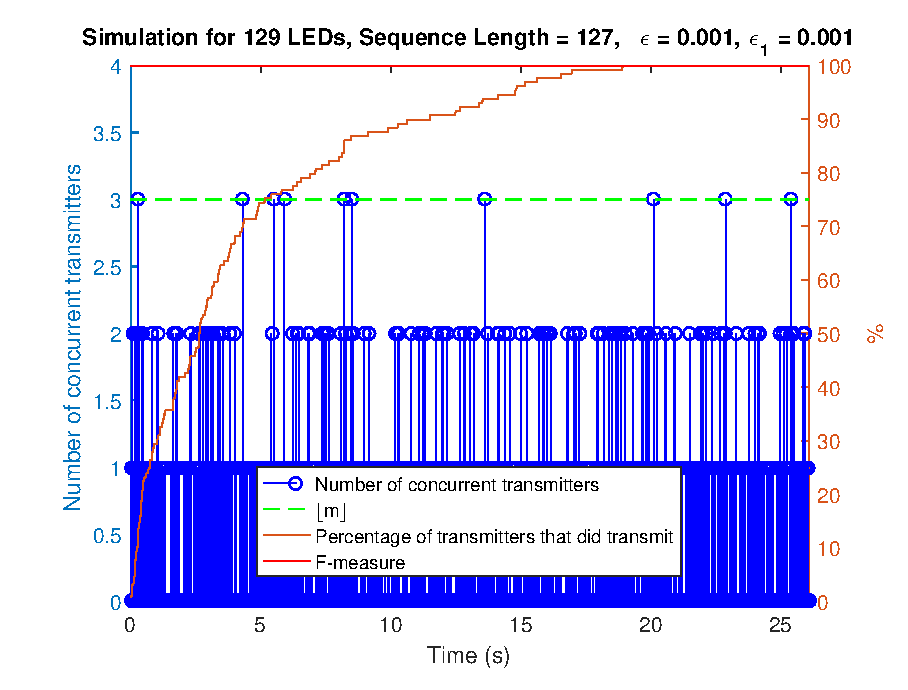
\includegraphics[width=0.8\textwidth]{simulation-2.eps}
		\end{figure}

		% In this simulation we still have the same number of transmitters, 129, but we require more precision and completeness.
		% We see that it takes more time to complete: around 26 seconds but 99 % of the transmitters have actually transmitted 
		% and only one time was there too much interference.


	\end{frame}











\end{document}
